\documentclass[11pt]{article}

% this is the template for an issue of the Data Engineering Bulletin
% % all packages used by any paper must be listed here
\usepackage{deauthor,times,graphicx, url, enumitem,listing ,minted}
\graphicspath{{figures/}}

% Carlos' Latex Packages
\usepackage[colorinlistoftodos]{todonotes}
% \setuptodonotes{inline}

\begin{document}
\title{Transparent Decisions: Selective Information Disclosure With Synthetic Data}
\author{
Carlos Gavidia-Calderon$^1$, Steve Harris$^2$, Markus Hauru$^1$, Carsten Maple$^1$, Iain Stenson$^1$, and \\ May Yong$^1$ \\~\\
$^1$The Alan Turing Institute \\
$^2$University College London
}
\date{\today} % Or specify a specific date
\maketitle
\begin{abstract}
The UK government and the public are interested to see the National Health Service (NHS) leverage data and artificial intelligence for the public good \cite{gov2022datasaves}\cite{Jones2022}. A major challenge is balancing the need between accessible healthcare data in order to boost research against the necessity of protecting patient privacy. We introduce SqlSynthGen (SSG), a method for generating synthetic relational datasets. SSG offers a human-readable, risk-guided approach to refining data fidelity while managing disclosure risk. This paper presents SSG, specifically focusing on its application for generating synthetic hospital patient data.
\end{abstract}

\section{Introduction}

Hospitals currently manage and produce large quantities of
patient data stored in relational databases. While hospital staff access this data for their clinical duties, other professional communities--- scientists, software engineers and educators --- necessarily follow lengthy processes to be granted access. Controls are in place to ensure patient data ---which is both sensitive and valuable~\cite{schomerus2022}--- is accessed for only legitimate reasons. Current practices involve drawing up employee contracts, implementing de-identification or anonymisation mechanisms to remove personal information, and accessing data only via trusted environments~\cite{harris2022}.

While protecting patient privacy is of utmost importance, denying all access to patient data hinders its potential. For instance, researchers can use data to improve diagnostic accuracy, refine our understanding of diseases, or develop personalised treatments~\cite{tucker2020}; software engineers and data scientists could develop infrastructure to support patient care and hospital operations~\cite{harris2022}; and patient data can be used to train the next generation of healthcare practitioners and researchers.

In order to both protect user privacy \emph{and} control access, current techniques are used, which include mechanisms like data agreements, de-identification or anonymisation, aggregation over the original data, and storing them in trusted research environments (TRE) for access by third parties. While these techniques provide an extra layer of protection, they are not exempt from vulnerabilities~\cite{near2021}. For example, de-identified data releases are still susceptible to linkage attacks. Aggregation requires releasing only aggregate population metrics, like counts or averages, but this still leaves outliers vulnerable to identification~\cite{tucker2020}. Instead of releasing \emph{real} patient data ---either partial or aggregate--- an option is to release \emph{synthetic} patient data. 

Synthetic data is data that is manufactured, as opposed to real data that is collected from real-life events and people. \emph{Synthetic data generators (SDG)} use algorithms to produce synthetic data entries while preserving statistical properties of the real dataset. There are multiple SDG approaches in the literature, each one targeting a specific data type, like tabular data or time-series data~\cite{DBLP:journals/corr/abs-2205-03257}.
SDGs can offer mathematical guarantees of the preservation of user privacy~\cite{Kopp2021MicrosoftSD, Cai2023} by incorporating differential privacy.

In this paper, we describe our work on developing a new SDG approach at the University College London Hospitals (UCLH) NHS Foundation Trust. Each year, UCLH admits 100,000 patients and stores their data in a relational database. Broadly, we discover that these are their requirements regarding their utilisation:

\begin{listing}[ht]
\begin{itemize}
    \item \textbf{REQ-1:} The synthetic datasets should be in the form of relational datasets for any given relational schema
    \item \textbf{REQ-2:} The generator can manufacture synthetic data by utilising aggregates and statistical properties extracted from real patients
    \item \textbf{REQ-3:} The names and values of aggregate data and statistical properties, as well as the methods used to compute them, are easily understandable by humans. 
\end{itemize}
\caption{Requirements for Synthetic Data Generation at UCLH Trust}
\label{lst:UCLH Requirements}
\end{listing}

We developed \textsc{SqlSynthGen}~\cite{repository} to meet these requirements\ref{lst:UCLH Requirements} over relational datasets, with multiple tables and foreign keys between them~\cite{Cai2023}.
\textsc{SqlSynthGen} is an open-source Python package that can replicate the database schema of a target database. Once the replica is in place, \textsc{SqlSynthGen} can generate synthetic samples at different levels of fidelity: from low-fidelity random values compliant with the database schema, to high-fidelity samples from probability distributions learned from real data.

\textsc{SqlSynthGen} uses a white-box approach where information extraction from real data are expressed as SQL queries in human-readable format, instead of black-box approaches like deep generative models with thousands of parameters~\cite{DBLP:journals/pami/Bond-TaylorLLW22}. For ensuring patient privacy, \textsc{SqlSynthGen} supports differential privacy to add quantifiable noise to aggregates and statistical properties.

\section{Sharing Patient Data}

This section starts by enumerating motivations for sharing patient data. An understanding of motivations is important because the requirements of appropriate data sharing mechanisms depend on this. Why we want to share data decides what minimum data needs to be shared, and this in turn defines the requirements to be met if the data is to be shared reasonably safely.

We then survey the current privacy preservation practices currently adopted to address the requirements. Hospital Trusts enable collaborators access to patient data through a variety of controlled, secure, and legally compliant data-sharing practices.  We show that these are  a) time-consuming, b) linked to inadequate privacy protection measures~\cite{near2021, tucker2020}, c) a cause of unnecessary friction to analysis~\cite{ODonovan2023}, d) unsuitable for scaling to large relational datasets, a format in which many patient datasets are stored or e) able to achieve high, explainable fidelity at the cost of time series data and limited scalability~\cite{Cai2023}.

\subsection{On the Benefits of Sharing Patient Data}

\paragraph{Enhancing Research Quality and Innovation:} 
Collaboration can lead to more comprehensive research studies, allowing healthcare practitioners and researchers to test hypotheses or observe trends across a broader dataset than what's available internally. How well a dataset represents the true distribution matters more than simply dataset size\cite{app11020796}. In the medical domain, where lack of data is a common occurrence, the amalgamation of diverse datasets has a better chance of representing true underlying distributions. This enhances the reproducibility and robustness of research findings.

\paragraph{Access to Specialised Expertise:} 
External collaborators bring specialised knowledge and skills that complement the in-house capabilities of a hospital. For example, collaborations with methodology researchers can lead to state-of-the-art data analysis and interpretation, thereby improving both method development and treatment outcomes. Software engineers and machine learning operations engineers can build customised cyber-physical infrastructure to support analysis of patient data in real time\cite{harris2022}.

\paragraph{Accelerating Medical Discoveries:}
By pooling resources and data between hospitals, research can proceed at a faster pace\cite{app11020796}, potentially leading to quicker discoveries in disease mechanisms, treatment effectiveness, and development of new therapies or medical technologies. Sharing patient data can facilitate the recruitment of participants for clinical trials, ensuring a diverse and adequate sample size. This can be crucial in studying rare diseases or sub-types of common diseases, especially in hospitals that offer specialisations not commonly offered elsewhere in the world. 

\paragraph{Expanding Research Funding Opportunities:} Collaborative research often has better chances of securing funding\cite{Vasan2021}. Funding bodies frequently encourage or require collaboration across institutions as a criterion for grants, viewing it as a way to maximise the impact of their investment.

\paragraph{Bench-marking and Quality Improvement:} Comparing data across institutions can help identify best practices and areas for improvement in patient care and management. This bench-marking is used to drive quality improvement initiatives within a hospital\cite{Werner2005}.

\paragraph{Education and Training} Collaborations provide educational opportunities to clinical research employees at hospitals, researchers and students at universities and research institutions, exposing them to different perspectives, methodologies, and cutting-edge research through joint ventures and knowledge exchanges.

\paragraph{Building Networks and Reputation:} Collaborations can enhance a hospital’s reputation in the medical and scientific community\cite{Vasan2021}. They extend the hospital’s influence and recognition, which can attract top talent and more collaborations in the future.

\subsection{Current Practices For Sharing Patient Data}

\paragraph{De-identification and Anonymisation of Patient Data:}
De-identification is the process of obscuring or replacing personal identifiers to prevent the direct association of data with an individual. Common de-identification methods include explicitly removing,  masking or pseudonymisation of direct identifiers, and  aggregating data to remove specificity eg. binning.  

Anonymisation aims to ensure that data cannot be linked back to an individual by any means. Anonymisation strips datasets of all personal identifying information but it is not provable when this has been achieved. Conservative measures will strip a lot of information thereby heavily affecting the value of the dataset, and we still cannot be certain that there is not some way to de-anonymise. 

For example, the removal of timestamps from a medical dataset as part of an de-identification or anonymisation process is performed because timestamps can be used to re-identify a patient by linking a patient's records over multiple de-identified datasets. The pattern of timestamps can disclose information about a patient's health, as well as their frequencies away from home.

However the stripping of timestamps from a medical dataset erases important information because medical information is highly time-contextual. Part of the richness of medical data is its time-series nature. Medical data that has been stripped of time stamps has reduced richness of data and is limited what can be learnt from it. 

Effectiveness of both de-identification and anonymisation techniques is highly dependent on context, which includes the dimensionality, volume, and statistical properties of data. Other important aspects that need to be considered include which types of applications or analyses the data are to be used for, whether the data will be released publicly or with additional access control, and whether the data are tabular, relational, or have longitudinal or transactional characteristics.

\paragraph{Trusted Research Environments:}

Trusted Research Environments (TREs) are an important part of the data sharing mechanism ecosystem. TREs are the secure infrastructure and governance model that allows researchers to access and analyse data; they are often used in conjunction with other data-sharing mechanisms.

TREs play a major role in controlling the data access levels. To begin with, data access is controlled through secure authentication and authorisation mechanisms. This means that only approved researchers can access the data, and they can only access specific datasets approved for their role and research projects. Activities on TREs are closely monitored and logged.

In addition, TREs provide both physical and virtual security. Data in TREs are often stored in physically protected facilities. Virtual security measures such as firewalls, intrusion detection systems and regular penetration testing maximise protection against external threats.  Finally, to ensure no privacy leakage, data egress from TREs is restricted. Researchers can analyse data within TREs but cannot take it out.

This means that working with data within TREs is far from a comfortable experience \cite{ODonovan2023}. In order to provide security measures, computational resources can be limited and the list of approved software packages for analysis is restrictive and not easily updated. There is significant process overhead generated by the need for detailed authentication into remote machines, activity logging, monitoring and compliance checks. There is a steep learning curve in working within a TRE, and new users are heavily dependent on support staff for technical assistance. Finally, the inability to egress data limits the sharing of interim findings and prevents close collaboration on ongoing data analysis.

\paragraph{Honorary contracts and data agreements:}

In order for non-hospital/clinical staff to work with medical data, they typically either need to become honorary employees of a trust or their current institution need to enter into a data sharing agreement with the trust. Both are lengthy and restrictive.

The process of obtaining an honorary contract typically begins with an initial inquiry and application to the relevant department or clinical group at the hospital. This is followed by credential verification and background checks, including border security investigations. Once these checks are satisfactorily completed, the relevant departments can grant approval. 

To get a data agreement signed between two institutions, the first step is to identify the need for data sharing, specifying what data will be shared and how it will be used. Next, security requirements for storing, protecting, and accessing the data must be agreed upon by both parties. All these elements need to comply with relevant regulations. Finally, the agreement must be reviewed by the legal and compliance teams of both institutions to ensure all requirements are met and all parties are protected.

\section{From Sharing Real Data to Sharing Synthetic Data}
Real data is recorded from real life events or organisms. Synthetic data is manufactured data, and can be synthesised to be random, structurally or type accurate, or they can mirror statistical properties of another dataset. In the last case, statistical properties can be directly or indirectly observed, to inform the manufacturing process. When any properties of one dataset is used to guide the manufacturing process of another dataset, the first dataset is referred to as the 'real' or 'original' data. In the use case presented in this paper, 'real' data is hospital patient data. Our manufactured data is commonly referred to as 'synthetic' data.

While manufactured patient data is not about real individuals, it is a fallacy to imagine that adoption of synthetic data in data sharing practices prevents disclosure of sensitive information. This section shows how synthetic data generators can manufacture outputs which disclose more, or less sensitive information, and how this affects the ways in which outputs can be used.

\subsection{Synthetic Data Generators}

Synthetic data generators (SDG) manufacture data. There is a tension observed in the process of manufacturing synthetic data which involves three factors: fidelity, utility and privacy. Fidelity measures the extent to which synthetic data resembles the real dataset. Utility is the measure of the usefulness of synthetic data to a given task. Privacy is a measure of the information disclosed about the real dataset during generation of the synthetic dataset. These three factors inform the manufacturing process and limit the ways its outputs can be used. Synthetic data which is very similar to the real dataset (high fidelity) risk leaking information about real patients (low privacy). Low fidelity datasets contains little real information so individuals are unlikely to be identified. 

However, low-fidelity or coarse-grained datasets can be useful, as utility is depending on the context or task. In some cases, low-fidelity datasets are valuable if they provide sufficient information for engineering applications e.g.\ software testing. When paired with real data, multi-fidelity datasets can reduce computational costs and prevent over-fitting in machine learning tasks \cite{Patra2020}\cite{Santoni2024}\cite{berkson2019}. Low fidelity datasets can remove blockers at the beginning of research for initial exploration, building pipelines, and testing models. These tasks can be conducted in a secure environment restricted to students and researchers, with scripts later ported to the hospital for training on real data if the initial analysis proves promising.

This means that there is a class of low-fidelity datasets that is useful in common research and engineering tasks. The benefits of using these datasets can be gained with little cost to patient privacy. 

\begin{figure}[ht]
\caption{Shows the range of fidelity for synthetic data. High fidelity data can result in higher utility, but also increased risk of identification.}
\centering

\includegraphics[width=0.8\linewidth]{figures/ONS.png}
\label{fig:Range of fidelity for synthetic data}
\end{figure}

Figure \ref{fig:Range of fidelity for synthetic data} shows the range of fidelity for synthetic data. In the context of healthcare relational datasets: 

\begin{itemize}
    \item \textbf{Structurally correct datasets} has the same column names, tables and relationships as real data. 
    \item \textbf{Valid datasets} imply that the values in the synthetic dataset are correct and valid, e.g.\ date of births are valid dates. 
    \item \textbf{Plausible datasets} imply that the relationship between values are realistic, e.g.\ a patient's date of death is not before their date of birth.
    \item \textbf{Multivariate plausible datasets} implies that the values are correlated across different variables, e.g.\ a male patient like likely to be both heavier and taller than a female patient. 
    \item \textbf{Multivariate detailed datasets} are more realistic than a multivariate plausible data set, but less than a replica of the real data. An example are rows of data showing that a patient with a diabetes diagnosis has more records of blood sugar readings than a patient with a broken bone.
\end{itemize}

\textit{NOTE: Carsten, can I have some help here please? Some words about state of the art generators and their applications and limitations would be really useful}

\subsection{Synthetic Data For UCLH NHS Trust}

University College London Hospitals National Health Services Foundation (UCLH NHS) Trust  is a pioneering institution within the UK, renowned for its treatment care and specialist services not widely available in other NHS Trusts. It is closely affiliated with University College London; this is a partnership that emphasises research and education, integrating medical research and teaching at the undergraduate and postgraduate levels directly into the clinical environment. 
As an institute that emphasises medical care, research and education, and as custodians of highly sensitive medical data, UCLH NHS Trust are in a position to leverage research capabilities to supercharge innovation if they can develop a process for thoughtful access to this data. 
However, consequences of accidentally releasing identifiable information include loss of individuals' privacy, loss of institutional prestige, as well as substantial legal fines.

\subsubsection{Problem Statement}

Machine learning (ML) infrastructure are deployed in hospitals to enable AI in healthcare delivery and administration. ML infrastructure supports tasks such as structuring data from electronic health records into a format that can be used as inputs to AI algorithms, deploying image analysis and predictive analysis tools, and presenting the results to healthcare practitioners in a timely and useful format.

To achieve these tasks, engineers who build the infrastructure need to gain an understanding of the data structures and data flow within the hospital. Researchers need to evaluate if target datasets meet their purposes for hypothesis testing, and are adequate in terms of quality and quantity. It is onerous to issue contracts to entire teams of engineers, researchers and students, but there are no other ways to share data with external collaborators. 

However, what engineers and researchers need when working on early stages of exploratory analysis to  understand data in terms of content, structure and data flow is information \emph{about} the data, not access to individual rows of data itself. Here is an  opportunity to frame the problem as: \emph{What information can be released about sensitive data, which is maximally beneficial to engineers and researchers, with minimal cost to patient privacy}?

\subsubsection{Requirements}

Listing \ref{lst:UCLH Requirements} enumerates the requirements of building synthetic data generators for UCLH Trust. This section expands on each requirement; the following section demonstrates how the design of SSG fulfils these requirements.


\paragraph{Produce relational datasets for any given schema:}

Many data holders, including hospitals, store patient electronic health records in relational databases. Data is often structured within complex schema that capture both single observations and time series data. These relational databases also include tables for vocabularies such as definitions of drugs, observations and diagnoses. 

Under this requirement, a minimally useful synthetic dataset must at the very least a) be structurally correct. That is, it will contain the same tables, columns, and data types as the real data, and b) meet foreign key constraints. In order to increase analytical value as shown in Figure 1, the synthetic generator will need to generate values which are valid and plausible, e.g. valid gender values and a plausible distribution of height and weight.  A multivariate plausible dataset will have values that correlate across multiple tables, e.g. the correlation between gender and height are represented across the `Demographic` and `Observation` tables. 

An additional complexity here is in generating synthetic time series data, e.g. blood pressure values every ten minutes for a patient in intensive care unit. In order to be multivariate plausible, the data needs to contain the correct frequencies for data collection as well as plausible values that depend on a patient's physiology. This is generated across multiple tables as well.  

\paragraph{To generate synthetic data using statistical properties computed from real patients}
Hospitals are mandated or encouraged by various information acts to release hospital information to the public. The main reasons for this are allowing insights into quality of care provided by public or insurance funds and to enable patients to make informed decisions regarding where to seek care based on hospital performance and specialisations\cite{Werner2005}. 

The type of information that is released in the public domain include quality of care indicators, patient safety data, readmission rates and service availability. This includes aggregate data about patient outcomes, infection rates, details on specialised services, bed occupancy, Accidents and Emergency (A\&E) wait times as well as statistical properties on patients returning for treatment within a period of discharge. This information is published regularly and does not compromise individual patient privacy.  

Synthetic data generators can use aggregate data and statistical properties of real data to generate datasets which are measurably closer to real data. A synthetic dataset generated using public information will not reveal any additional patient information beyond what is already publicly available.

\paragraph{Ensure that the names and values of aggregate data and statistical properties, as well as the methods used to compute them, are easily understandable by humans.}

% \todo{Markus: Could the content in this section be restructured so that it wouldn't start with differential privacy? Something like synthetic data is complex and communicating about its privacy aspects is hard, and on top of that we want to use differential privacy which makes it extra hard.}

Aggregates and statistical properties are well-understood mathematical concepts. A comprehensive explanation of such information extracted from real patients datasets for the purpose of generating synthetic data should cover the following three points:

\begin{enumerate}
    \item \textbf{Extracted Information}: Detail what specific information about patients has been extracted.
    \item \textbf{Computation Process}: Explain how this information is computed.
    \item \textbf{Usage for Synthetic Data}: Describe how this information is used to shape the synthetic data.
\end{enumerate}

Providing this explanation in a single, human-readable source ensures consistency and prevents obsolescence across multiple data generation iterations. This offers a clear audit trail of the generation process and helps identify the disclosure risks of its outputs.

The concept of synthetic data is complex, people may not understand how data that does not represent real individuals still needs privacy considerations. It is furthermore difficult to understand how the application of differential privacy to aggregates and statistics can provide additional protection. 

Differential privacy (DP) \cite{DworkR14} is the gold standard that protects individuals within a dataset while still allowing for the useful analysis of the aggregate data. Its internal mechanics  of noise addition for the purpose of privacy preservation can leave users without a clear understanding of its outputs and how to interpret them correctly. 

The application of differential privacy to synthetic data compounds the explanations' complexities. There is a struggle to understand how DP offers probabilistic but not absolute guarantees. Explaining this to custodians of highly sensitive data is difficult because privacy is expected but not always technically feasible. 

However, this is an important discussion, there is a necessary understanding to be achieved here because the interplay between privacy and utility governs the results of a differentially private synthetic data generator. The only people who can take the responsibility for managing the balance between privacy and utility are the data custodians.
 
\section{Generating Synthetic Data Using \textsc{SqlSynthGen}}

\textsc{SqlSynthGen} (SSG) is a software package that we developed to meet the requirements outlined in Section 3.3. When connected to an existing relational database, SSG builds a new empty database with the same schema. It copies over the non-sensitive data, such as look-up tables, and generate structurally correct synthetic data with random values. Optionally, SSG can refine these synthetic values using aggregates and statistical properties. SSG can apply differential privacy to obfuscate the true values of these properties in a measurable way. The new database is then populated with these synthetic values.  

\subsection{Technical Overview}

SSG's default output dataset is structurally correct and has no disclosure risk. These are datasets that sit on the far left end of the spectrum in Figure \ref{fig:Range of fidelity for synthetic data}. No information about the real dataset has been disclosed, beyond the structure in which they are stored. This can already be useful e.g. for building software testing modules and pipe-lining scripts, and can be safely released if vocabularies and schema can be shared. \textbf{\textit{This meets REQ-1: Produce relational datasets for any given schema.}}

SSG can be further configured to generate synthetic data that (in reference to Figure \ref{fig:Range of fidelity for synthetic data}), can be as sophisticated as multivariate plausible data. This is achieved by allowing the user to define SQL statements that extract aggregate statistics and statistical properties from the real data. These extracted values are then used to shape the distributions and marginals of the synthetic data. \textbf{\textit{This meets REQ-2: To generate synthetic data using statistical properties computed from real patients.}} 

As part of its process, SSG generates a human-readable audit trail that details the entire data generation process. This includes what information was extracted from real data, the methods used for extraction, the computed results, and how these values were injected into the synthetic data generation. The audit trail is a human readable file whose contents are incorporated directly into the SDG process. \textbf{\textit{This meets REQ-3: Ensure that the names and values of aggregate data and statistical properties, as well as the methods used to compute them, are easily understandable by humans.}}

SSG pipeline design enables the selective production of synthetic datasets with varying levels of fidelity. Users control the shaping of synthetic data by specifying which information is extracted from real data, how it is computed, and how it is utilized. SSG’s configuration supports agile development, allowing for incremental fidelity improvements as needed, while maintaining transparency, auditability, and control over privacy risks at every stage. Additionally, users have the option to apply differential privacy to protect the marginals extracted from the source data.

\begin{figure}[ht]
\centering
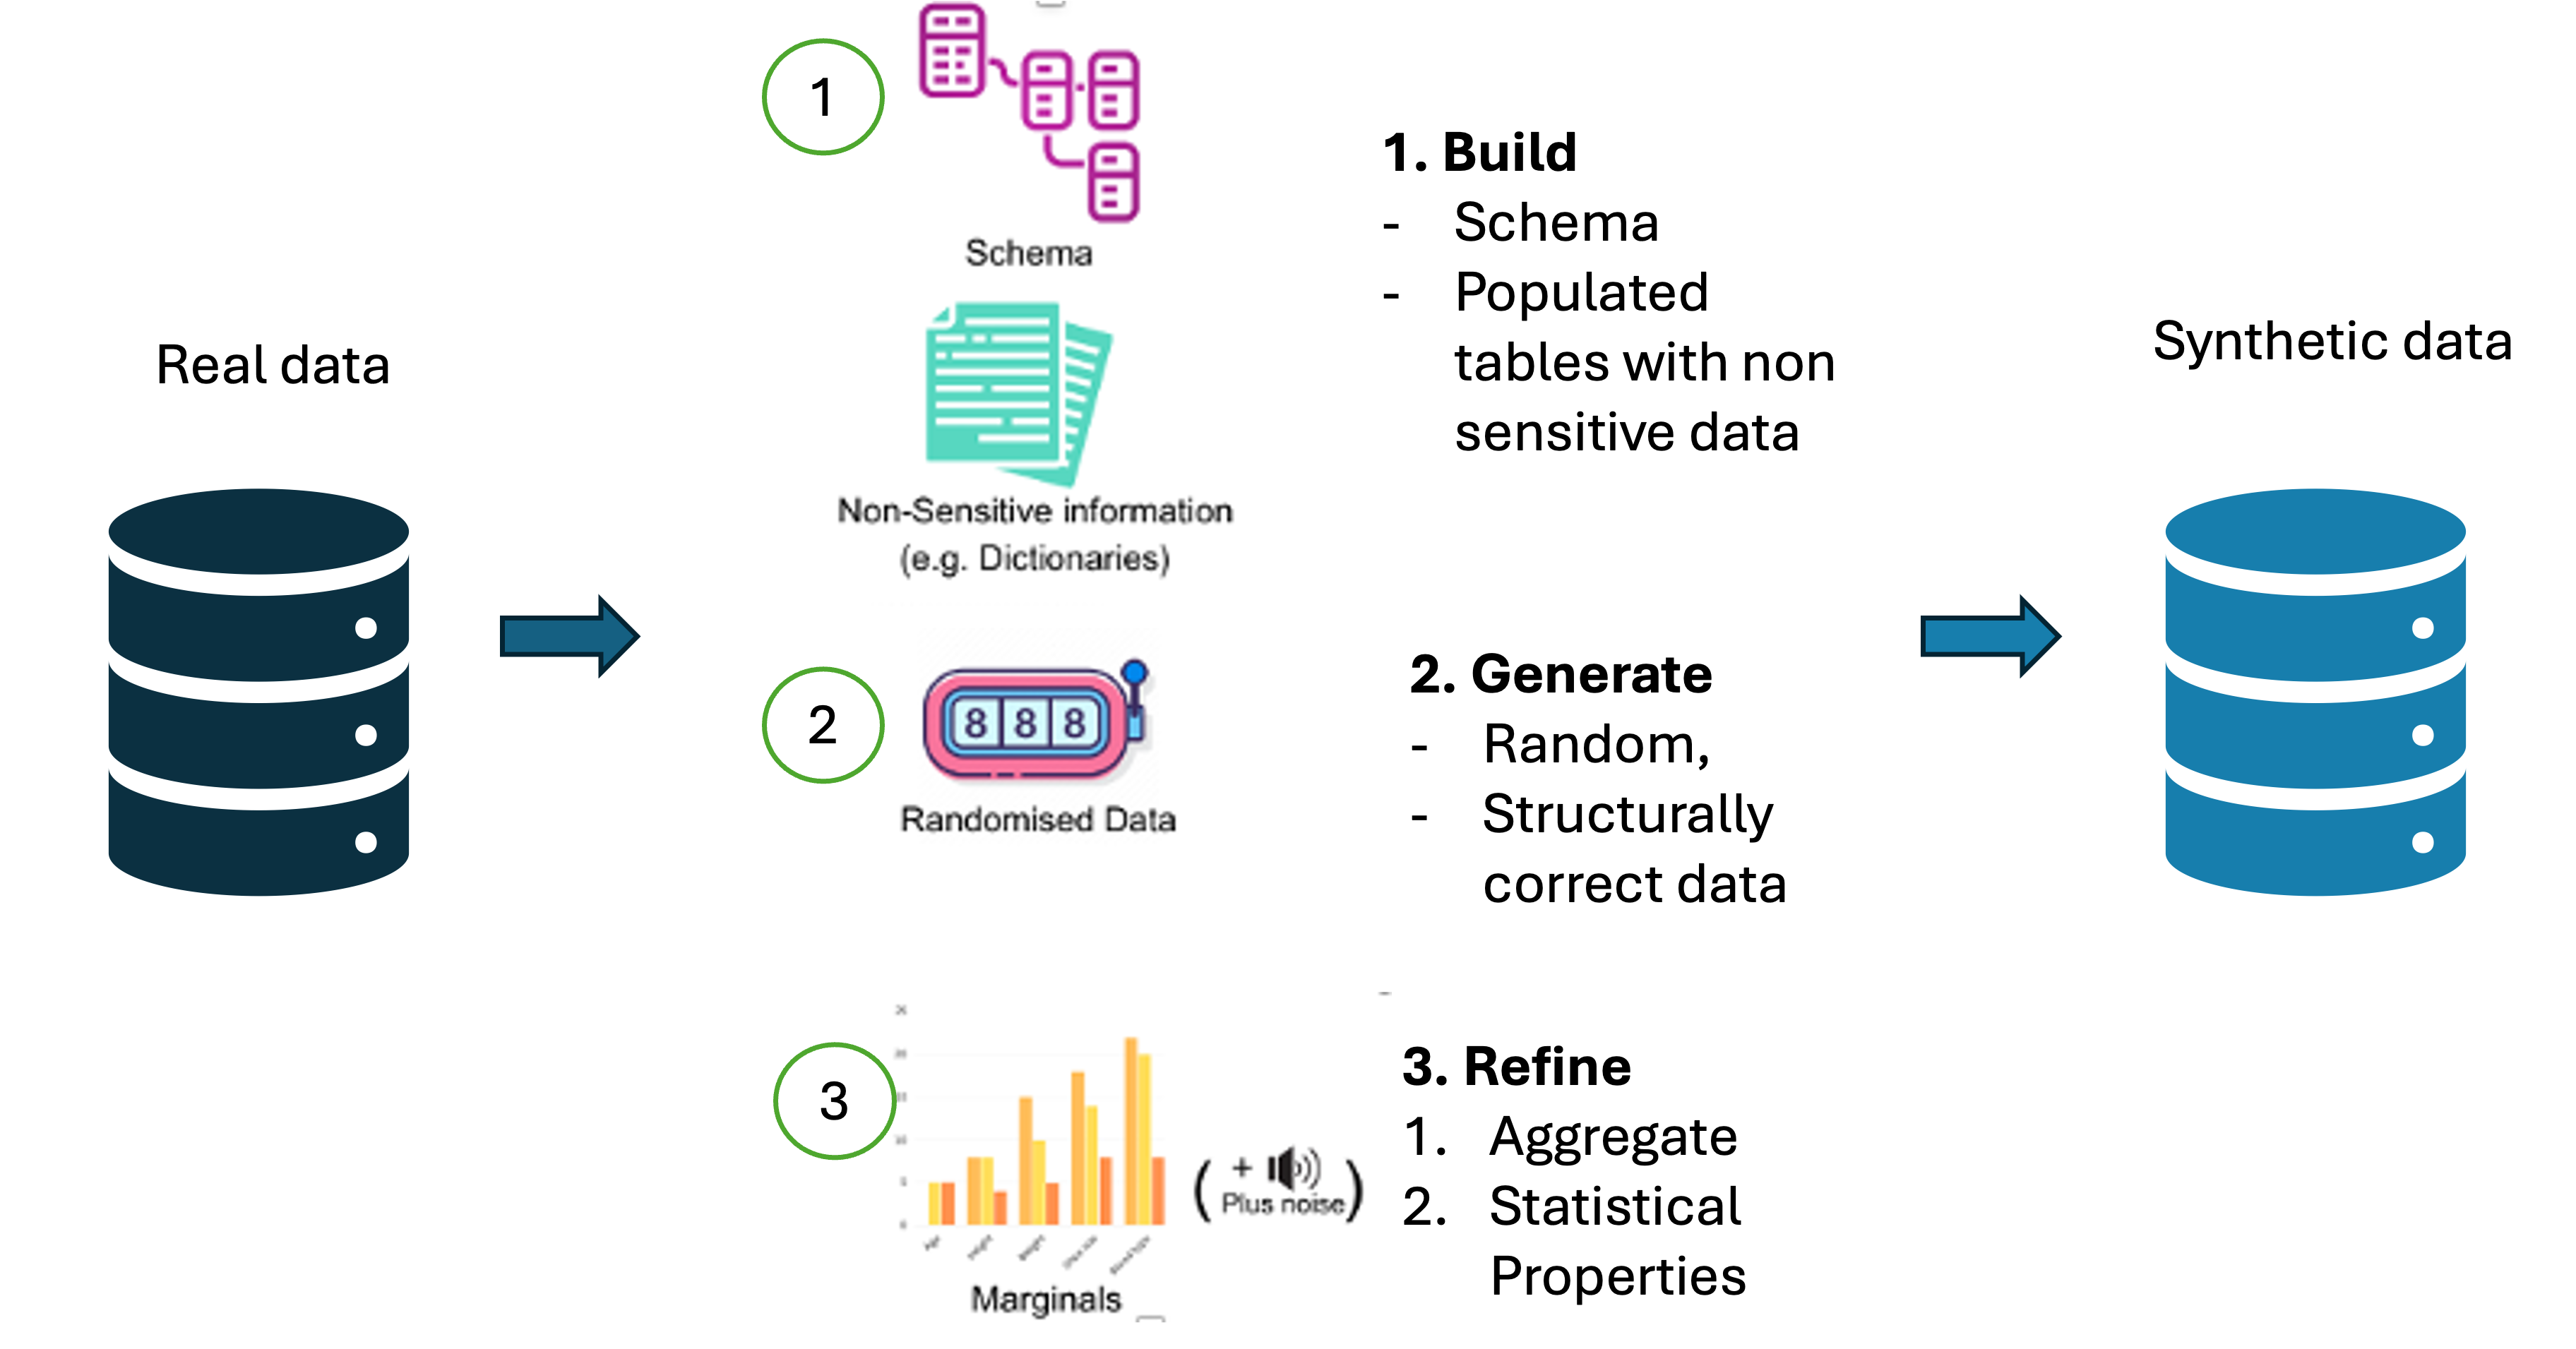
\includegraphics[width=0.8\linewidth]{figures/Process.png}
\caption{The processes of SQLSynthGen in order}
\label{fig:SSG Process}
\end{figure}

In order to support this design, SSG's process for generating synthetic relational datasets can be broken into three separate steps, as shown in Figure \ref{fig:SSG Process}. They are as follows:

\begin{enumerate}
    \item SSG \textbf{builds} a new database to store synthetic data. This new database will be populated by synthetic data generated in the next steps. Look-up tables which do not have any privacy concerns are copied over entirely, to maintain foreign key constraints.
    \item By default, SSG \textbf{generates} random but structurally correct data. 
    \item As an option, SSG can \textbf{refine} random values for higher accuracy by using extracted statistics from real data, with or without DP. For example, mean of height by age and gender can be extracted from real patients and the correlation be used to generate higher fidelity data.
\end{enumerate}

For more information and tutorials about SQLSynthGen, please refer to our repository at \url{https://github.com/alan-turing-institute/sqlsynthgen}. Our repository \cite{repository} contains installation instructions, comprehensive documentation and trouble shooting guides to help get started with the software. The repository also contains a simple tutorial using a Kaggle dataset \cite{airbnb} as well as an advanced example based on the Observational Medical Outcomes Partnership (OMOP)\cite{omop}, which provides a standardised data model for observational healthcare data. 

In the following sections, we demonstrate the use of SSG in creating synthetic data based on a publicly available AirBnB Kaggle dataset \cite{airbnb}.

\subsection{Building a Replica of a Real Dataset}

In this example, let us consider that our dataset is contained in a database called `airbnb` in a local PostgreSQL instance. We want to port the schema to a new `airbnb\_synthetic` database, and populate the `airbnb\_synthetic` database with synthetic rows that mirror some of the statistical properties of the `airbnb` dataset.

\paragraph{Build schema tables:}

We connect to the real dataset by setting connection credentials in the relevant environment variables. We run a series of commands \mintinline{bash}{sqlsynthgen make-tables}, \mintinline{bash}{sqlsynthgen create-tables}, and \mintinline{bash}{sqlsynthgen make-generators} to auto-generate two Python files. 

The first file, `orm.py`, outlines the structure of the PostgreSQL `airbnb` dataset by mapping each table in 'airbnb' to a corresponding Python class. Each column in these tables is represented as a class field. This mapping is generated using SQLAlchemy\cite{sqlalchemy}, which is a SQL toolkit and Object-Relational Mapping (ORM) library for Python. By using SQLAlchemy in SSG for mapping, users do not need to perform any additional configuration to describe the schema of the real dataset. The `orm.py` file serves as a foundation for building a new `airbnb\_synthetic` PostgreSQL database, complete with the necessary tables, columns and data types. Listing \ref{lst:orm.py} shows a snippet from `orm.py` that demonstrates how the  `users` table from the `airbnb`  dataset is mapped as a Python class.

\begin{listing}[H]
\begin{minted}[
    % gobble=2,
    frame=single,
    linenos
  ]{Python}
class User(Base):
    __tablename__ = "users"

    id = Column(String, primary_key=True)
    date_account_created = Column(Date)
    ...
\end{minted}
\caption{Section of PostgreSQL table `user` represented as a Python class}
\label{lst:orm.py}
\end{listing}

\paragraph{Copy over lookup tables}

A lookup table, or a vocabulary is a table used to store a predefined set of values that are referenced by other tables. They contain finite and static set of values such as codes, names of categories or descriptions. Look-up tables are a good practice adopted help normalise databases by removing redundancy and enabling efficient data management. They work by using foreign key constraints to ensure values in related tables are consistent and valid. These foreign key constraints need to be satisfied when generating synthetic data in relational datasets. On their own, vocabularies provide only limited utility, as the more interesting aspects of the data are usually found in the non-vocabulary tables. 

The fidelity of the synthetic dataset can be improved by ensuring the vocabulary tables have perfect fidelity from the beginning, as they do not raise privacy concerns, although some vocabularies are copyright-protected. In this section, we demonstrate how SSG addresses vocabulary tables by copying them in their entirety, thereby eliminating the need for synthesising.

First we specify vocabulary tables in a \texttt{config.yaml}; the listing \ref{lst:vocabulary-config.yaml } below denotes `countries` as a vocabulary table. All values in denoted vocabulary tables are copied to an auto-generated \texttt{.yaml} file. Listing \ref{lst:countries.yaml} shows a snippet of data from the `countries` table which has been copied to a auto-generated \texttt{countries.yaml} file.

\begin{listing}[H]
\begin{minted}[
    gobble=2,
    frame=single,
    % linenos
  ]{yaml}
    tables:
        countries:
            vocabulary_table: true
\end{minted}
\caption{A yaml section to demarcate table 'countries' as a vocabulary table}
\label{lst:vocabulary-config.yaml }
\end{listing}

\begin{listing}[H]
\begin{minted}[
    gobble=2,
    frame=single,
    % linenos
  ]{yaml}
    - country_destination: AU
      destination_km2: 7741220
      destination_language: eng
        :
    - country_destination: CA
      destination_km2: 9984670
      destination_language: eng
      distance_km: 2828.1333
        :
\end{minted}
\caption{Example of data rows copied from `countries` vocabulary table}
\label{lst:countries.yaml}
\end{listing}

The primary reason for copying vocabularies this way is to maximise transparency for auditing purposes. Data holders can audit each value extracted from the real dataset, before creating any synthetic data. Note that we have to be careful in making sure that the tables marked as vocabulary tables truly do not hold privacy sensitive data, otherwise catastrophic privacy leaks are possible, where the original data is exposed raw and in full. 

The downside of this approach is clear when scaling up to address vocabulary tables which are very large. Therefore our generator pipeline is modular to ensure that vocabularies need only be copied once when creating more rows to add into a synthetic dataset. 

\paragraph{Generate Random Values that are Structurally Correct}

The second auto-generated file, `ssg.py`, contains Python code that generates random values matching the data types defined by the Python classes. This human-readable Python code serves as part of the audit trail, demonstrating how values for populating each table column are generated. For complex schemas with multiple tables and columns, the generator code for each column is easily identifiable and can be customised independently of rest of the generator. 

Listing \ref{lst:ssg.py} demonstrates the auto-generated Python code for generating `id` and `date\_account\_created` values for the `User` table. `id` is assigned generic, password-like values, and `date\_account\_created` is assigned a random date value.

\begin{listing}[H]
\begin{minted}[
    % gobble=2,
    frame=single,
    % linenos
  ]{Python}
class usersGenerator:
    num_rows_per_pass = 1

    def __init__(self, src_db_conn, dst_db_conn):
        pass
        self.id = generic.person.password()
        self.date_account_created = generic.datetime.date()
        ...
\end{minted}
\caption{A Python class for generating synthetic id and date\_account\_created values for Postgres table `User`}
\label{lst:ssg.py}
\end{listing}

\paragraph{Refine values using aggregate statistics}

The default behaviour of SSG is to generate syntactically correct, random values. This section shows how we incorporate aggregate and statistical properties of real data in order to generate synthetic data that retain those properties. 

We demonstrate an example to generate normally distributed synthetic values to populate a `users.age` column, with reference to the mean and standard deviation values of the real data. The user begins by defining SQL statements in the `age\_stats` section of a `config.yaml` file. This is demonstrated in listing \ref{lst:define sql and row generator in config.yaml}. SSG uses the credentials provided to authenticate to the database and execute SQL statements to compute the required values. Computed values are recorded in an auto-generated \texttt{src-stats.yaml} file, demonstrated in listing \ref{lst:age_stats src-stats.yaml}. These can be can be referenced by the Python data generators. Listing \ref{lst:provider-function} shows the Python provider function that generates a distribution of values to meet the statistical properties computed and recorded in `config.yaml` and `src-stats.yaml`.

\begin{listing}[H]
\begin{minted}[
    gobble=2,
    frame=single,
    % linenos
  ]{yaml}
    src-stats:
        - name: age_stats
        query: >
        SELECT AVG(age)::float AS mean, STDDEV(age)::float AS std_dev
        FROM users
        WHERE age <= 100
    tables:
        users:
            row_generators:
              - name: airbnb_generators.user_age_provider
                kwargs:
                  query_results: SRC_STATS["age_stats"]
                columns_assigned: age
\end{minted}
\caption{A section of the config.yaml file that shows an SQL statement to compute mean and average of column `users.age`, with results stored as `age_stats` }
\label{lst:define sql and row generator in config.yaml}
\end{listing}

\begin{listing}[H]
\begin{minted}[
    gobble=2,
    frame=single,
    % linenos
  ]{yaml}
    age_stats:
    - mean: 36.54434029695572
      std_dev: 11.708339792587486
\end{minted}
\caption{Example of mean and standard deviation values computed from `users.age` column}
\label{lst:age_stats src-stats.yaml}
\end{listing}

\begin{listing}[H]
\begin{minted}[
    gobble=0,
    frame=single,
    % linenos
  ]{Python}
    import random
    def user_age_provider(query_results):
        mean: float = query_results[0]["mean"]
        std_dev: float = query_results[0]["std_dev"]
        return random.gauss(mean, std_dev)
\end{minted} 
\caption{A provider function }
\label{lst:provider-function}
\end{listing}

The primary reason for extracting information using SQL statements and documenting it in `config.yaml` is to maximise transparency for auditing purposes. Similar to vocabularies, users can audit information that is disclosed about real data by reviewing the human-readable `config.yaml` and `src-stats.yaml` files. Multiple properties, such as marginals, percentiles, and skewness, can be used simultaneously to enhance the fidelity of synthetic data. These computations can be resource-intensive with large datasets. To address this, the SSG generator process is modularised: properties are computed and stored once, allowing subsequent generators to  reference these values, which will be reliable provided the real dataset has not changed significantly.

\paragraph{Introduce differential privacy into aggregate statistics:}

\emph{Differential privacy} is arguably the most popular technique for providing privacy guarantees on SDGs.
Let us imagine two datasets:

\begin{itemize}
    \item A synthetic dataset $B$ generated \emph{with} information of person $X$.
    \item A synthetic dataset $A$ generated \emph{without} information of person $X$.
\end{itemize}

If both datasets were generated using a differentially-private \emph{mechanism}, performing a query on dataset $A$ should provide the same, or almost the same, result as performing the same query on dataset $B$~\cite{Kopp2021MicrosoftSD}.
Differentially private mechanisms hide the presence or absence of person $X$ ---or one any individual--- in the dataset, which implies strong protection of their privacy~\cite{near2021}.
To accomplish this, these mechanisms inject random noise to the synthetic data.
The amount of noise is a function of the privacy parameter epsilon $\varepsilon$ that measures how similar the datasets $A$ and $B$ are required to be. $\varepsilon$ needs to be chosen carefully to provide the required privacy guarantee.

Generating synthetic data in a differentially private way usually requires 3 steps: 1) \emph{select}, or choose, some queries over the original data, 2) \emph{measure}, or execute, those queries using a differentially private mechanism, and 3) \emph{generate} synthetic data using these measurements~\cite{DBLP:journals/pvldb/McKennaMSM22}.

\textsc{SqlSynthGen} enables the \emph{select} and \emph{measure} steps by supporting differentially private SQL queries in `src-stats.yaml`  (Listing \ref{lst:dp-queries}).

\begin{listing}[H]
\begin{minted}[
    gobble=2,
    frame=single,
    % linenos
  ]{yaml}
    src-stats:
      - name: age_stats
        dp-query: >
          SELECT AVG(age) AS mean, STDDEV(age) AS std_dev
          FROM query_result
        epsilon: 0.5
        delta: 0.000001
        snsql-metadata:
          max_ids: 1
          id:
            type: string
            private_id: true
          age:
            type: float
            lower: 0
            upper: 100
\end{minted}
\caption{A differentially-private SQL query. }
\label{lst:dp-queries}
\end{listing}

Internally, \textsc{SqlSynthGen} uses \textsc{SmartNoise SQL}~\cite{allen2020opendp} to execute differentially private queries.
As seen in Listing \ref{lst:dp-queries}, \textsc{SmartNoise SQL} needs additional information besides the SQL query for applying a differentially private mechanism, including the privacy parameter epsilon $\varepsilon$.
Regarding the final \emph{generate} step, the query results are made available to provider functions ---like the one in Listing \ref{lst:provider-function}--- so \textsc{SqlSynthGen} users can use these measures for data generation. 

\section{Plans for Implementation}
% Suggest how the software might sit within the hospital's existing systems and workflows. (Not yet, but plans?)
% Describe any challenges anticipated during the implementation phase. Include feedback from the hospital staff and patients, if available, to provide a comprehensive view of the challenges. (Patient engagement group?) (Steve?)


\section{Discussion}
% Explore the broader implications of your findings for similar institutions or settings (any relational tables, HSBC?)
% Address any limitations of your study or software and suggest areas for future research or development. (SECURITY!!!)

\section{Conclusion}
Summarise the key points made throughout the paper, reiterating the software's role in addressing the hospital's challenges.
Reflect on the broader contributions of work to the field of healthcare IT.

\bibliographystyle{plain}
\bibliography{references}

\end{document}
